\documentclass[main.tex]{subfiles}
\begin{document}


\chapter{Double beta decay}
 

\begin{flushright}
\textit{Nothing contributes so much to tranquillize the mind \\
as a steady purpose, a point on which the soul \\
can focus its intellectual eye.}\\
Mary Shelley, \textit{Frankenstein}.
\end{flushright} 


\NI Since the neutrino existence prediction in 1930 and their first detection in 1956, many works have been realized to understand their properties. One of the more important achievements being the discovery of their oscillations, proving their non-zero mass which is a first indication of physics beyond Standard Model. 


\bigskip 


\NI After many years of neutrino research some fundamental parameters are still unknown. Experimental searches for neutrinoless double beta decay (0$\nu\beta\beta$) are one of the most active research topic in neutrino physics. Its observation is in fact of major importance since it will prove the Majorana nature of neutrinos and may give access to their absolute mass scale.


\bigskip


\NI Before to discuss the 0$\nu\beta\beta$ decay in Section~\ref{sec:0nubb}, some elements about radioactivity and double beta decay are introduced in Sections~\ref{sec:radioactivity} and~\ref{sec:2nubb}. Section~\ref{sec:ExperimentalSearches} describes the different approachs to experimentally detect the 0$\nu\beta\beta$ decay. A status of different experiments searching for 0$\nu\beta\beta$ decay is given in Section~\ref{sec:Status0nubb}.
  

\section{The radioactivity}\label{sec:radioactivity}


\NI Discovered in 1896 by Henri Becquerel, while working with phosphorescent materials, and confirmed later by Marie Curie, radioactivity is a physical process in which an unstable isotope loses energy by emitting radiation. Depending on the kind of radiation, the radiative decays have been sorted in 3 types : $\alpha$, $\beta$ and $\gamma$. Radioactivity is a natural phenomenon which can also be provoked (artificial radioactivity).


\bigskip


\NI At the level of a single atom, a radioactive decay is completely random. Even if we know since how long the isotope exist, it is not possible to predict when the decay will occur. But, in case of a collection of atoms, laws of statistics can be applied. The number of remaining (not decayed) isotopes at a certain time, N(t), can be estimated in terms of their decay constant ($\lambda$) or half-life ($\text{t}_{\text{1/2}}$ or T$_{\text{1/2}}$), and N$_\text{0}$, number of atoms in the initial sample : 


\begin{equation}
\text{N(t) = N}_\text{0}~\text{e} ^{-\lambda\text{t}}
\end{equation}


\NI with the relation : T$_{\text{1/2}}$ = ln(2)/$\lambda$. The time elapsed between the initial moment and the moment when it remains half of the initial sample is called the half-life. Half-lives of known isotopes vary widely, from more than 10$^{\text{19}}$ years ($^{\text{209}}$Bi), to 10$^{\text{-23}}$ seconds for highly unstable ones.


\subsubsection{Alpha decay}


\NI Alpha ($\alpha$) decay is a kind of radioactive decay in which an heavy nucleus emits a helium nucleus ($\alpha$ or $^{\text{4}}_{\text{2}}$He), for example, $^{\text{214}}$Po decays to form $^{\text{210}}$Pb :


\begin{equation}
 ^{\text{214}}\text{Po} \rightarrow  ^{\text{210}}\text{Pb} + \alpha
\end{equation} 


\NI Because it is a two-body reaction, the $\alpha$-particle is mono-energetic and at the order of~MeV (Q$_{\alpha}$ = 7.8~MeV in case of $^{\text{214}}$Po). Alpha decay occurs in heavy nuclei and governed by nuclear and electromagnetic interactions. The potential barrier due to the nuclear force is too important to be overcome by the electromagnic force. Only quantum tunnelling allows the emission of an alpha particle by the nucleus.


\subsubsection{Beta decay}


\NI A beta ($\beta$) decay transmutes a nucleus to a different element with emission of a $\beta$-ray (electron or positron) always accompagnied by neutrino or anti-neutrino. This decay is mediated by the weak force and can happen in 3 separate forms :


\begin{itemize}

\item $\beta^-$ : a neutron converts to a proton, an electron, and a anti-neutrino are emitted, 
\begin{equation}
\text{n} \rightarrow \text{p} + \text{e}^- + \bar{\nu}_\text{e}
\end{equation} 


\item $\beta^+$ : a proton converts to a neutron, an positron, and a neutrino are emitted, 
\begin{equation}
\text{p} \rightarrow \text{n} + \text{e}^+ + \nu_\text{e}
\end{equation} 


\item Electron capture (EC) : an atomic electron is captured by its nucleus, resulting in the emission of a mono-energetic neutrino,
\begin{equation}
\text{p} + \text{e}^- \rightarrow \text{n} + \nu_{\text{e}}
\end{equation}  

\end{itemize}


\bigskip


\NI For the isotopes where the $\beta^+$ decay is possible, a competition exists with the electron capture process. The captured electron leaves a hole in the atomic orbital. The reorganisation of the remaining electrons is accompanied by a cascade of photons, so the electron capture is usually accompanied by low energy X-rays and/or Auger electrons .

 
\subsubsection{Gamma ($\gamma$) decay}


\NI Just after the $\alpha$ or $\beta$ emission, the nucleus often reach an excited state of the daughter nucleus. It can then decay to a lower energy state by emitting one or more $\gamma$-ray(s). For example, after a $\beta$ decay, $^{\text{60}}\text{Po}$ reaches the excited state of $^{\text{60}}\text{Ni}$ ($^{\text{60}}\text{Ni}^\ast$) which emits 2 $\gamma$-ray at 1.17~MeV and 1.33~MeV : 


\begin{equation}
^{\text{60}}\text{Ni}^\ast \rightarrow ^{\text{60}}\text{Ni} + \gamma~\text{(1.17~MeV)} + \gamma~\text{(1.33~MeV)}
\end{equation}


\NI The emission of a $\gamma$-ray from an excited nucleus is a very fast process (at the order of 10$^{\text{-12}}$ seconds). 


\section{Two neutrino double beta decay}\label{sec:2nubb}


\subsection{Forbidden $\beta$ decays}


\NI All $\beta$ decays involve emission of particle and loss of energy, $\beta$ decay can only occur if the initial mass of the nucleus with A~nucleons and Z~protons, $\mathcal{M}$(A,Z$_\text{i}$), is greater than the final nucleus mass, $\mathcal{M}$(A,Z$_\text{f}$) : $\mathcal{M} \text{(A,Z}_\text{i}) > \mathcal{M} \text{(A,Z}_\text{f})$.


\bigskip


\NI As shown in Figure~\ref{fordiddenBetaDecay}, the $\beta$ decays (a) $\rightarrow$ (b) and (b) $\rightarrow$ (c) are allowed. Isotopes such as (c) are not completely stable but they can not decay by $\beta$ emission. To reach a stable state, they can undergo a neutrino double beta decay (2$\nu\beta\beta$). Note that it is theorically possible for the isotope (a) to directly decay to (c) by a 2$\nu\beta\beta$~decay, but this decay would not be observed since the decay rate of $\beta$~decay is far much shorter than 2$\nu\beta\beta$~decay.


\begin{figure}[h!]
\begin{center}
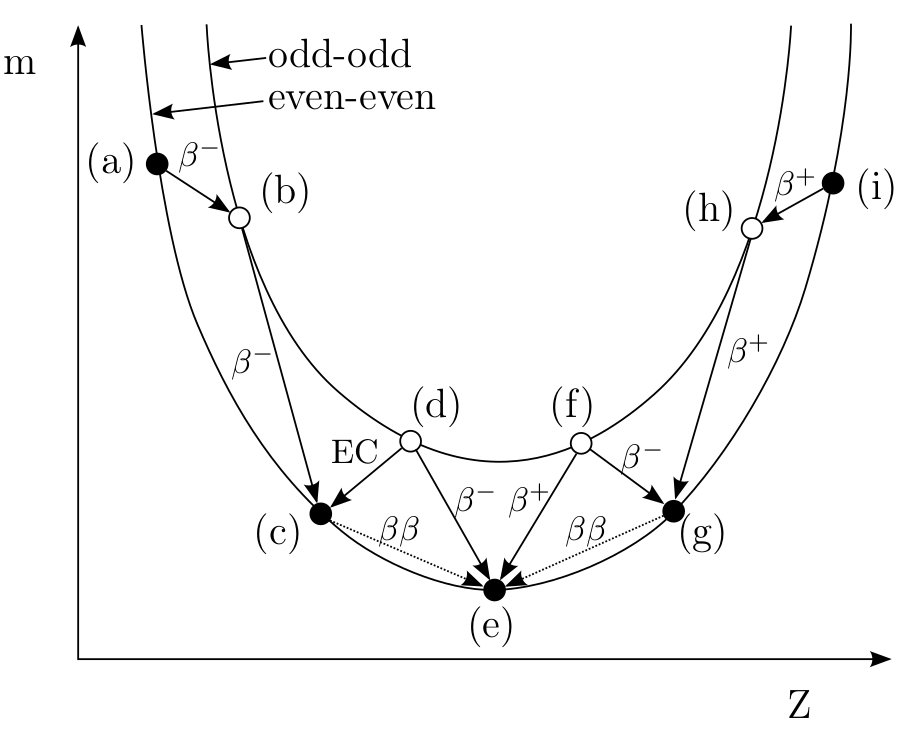
\includegraphics[scale=0.24]{pictures/Chap2/forbiddenBetaDecay.png}
\caption{Mass excess according the atomic number Z. The odd-odd isotope (a) can decay to the even-even isotope (b) via a $\beta$ decay. This daughter nucleus undergoes a beta decay to reach (c). The isotope (c) can not decay to (d) due to the energy conservation. To become more stable, only a 2$\nu\beta\beta$ decay is possible.}
\label{fordiddenBetaDecay}
\end{center}
\end{figure}


\subsection{Phenomenology}


\NI The 2$\nu\beta\beta$~decay is a 2$^{\text{nd}}$ order process allowed in the Standard Model. Figure~\ref{2nubbFeynman} presents its Feynman diagram.  Its existence have been proposed by Goeppert-Mayer in 1935~[ref]. So, it is a rare nuclear process in which 2$\beta^{-}$ (or 2$\beta^{-}$) happens simulataneously~: 


\begin{equation}
\mathcal{N} (\text{A,Z}) \rightarrow \mathcal{N} (\text{A,Z+2}) + \text{2e}^- + \text{2}\bar{\nu}_{\text{e}} 
\end{equation}

\begin{equation}
\mathcal{N} (\text{A,Z}) \rightarrow \mathcal{N} (\text{A,Z-2}) + \text{2e}^+ + \text{2}\nu_{\text{e}} 
\end{equation}


\bigskip


\NI Since the antineutrinos carry away a part of the energy, the total energy of the emitted electrons is a continuous spectrum with an end-point at the nuclear transition energy, Q$_{\beta\beta}$, defined as :


\begin{equation}
\text{Q}_{\beta\beta} = \mathcal{M}_\text{i} - (\mathcal{M}_\text{f} + \text{2m}_\text{e})
\end{equation}


\bigskip


\NI where m$_\text{e}$ is the electron mass. The shape of this spectrum is shown in Figure~\ref{bbDecaySpectrum}. The half-life of the decay can be written as : 


\begin{equation}
(\text{T}_{\text{1/2}}^{\text{2}\nu})^{\text{-1}} = \text{G}_{\text{2}\nu}(\text{Q}_{\beta\beta}, \text{Z}) \times |\text{M}_{\text{2}\nu}|^\text{2}
\end{equation}


\bigskip


\NI where G$_{\text{2}\nu}$ is the phase space factor that can be well calculated analytically and M$_{\text{2}\nu}$ is the nuclear matrix element (NME) for the decay. The computation of the NME are not trivial and are strongly model-dependent. More details about NME will be given in Section~\ref{sec:NME}.



\begin{figure}[h!]
\begin{center}
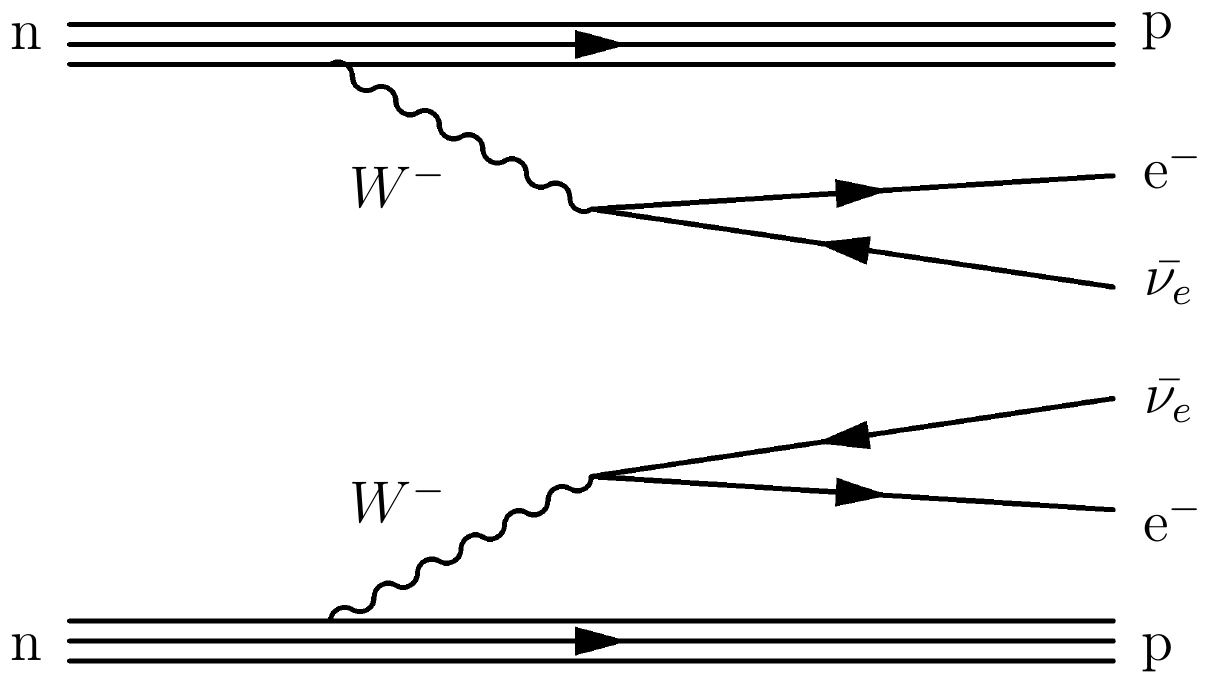
\includegraphics[scale=0.18]{pictures/Chap2/2nubb_Feynman.png}
\caption{Feynman diagram for 2$\nu\beta\beta$ decay. In this second order process, 2 neutrons decay simultaneously (2n $\rightarrow$ 2p + 2e$^-$ + 2$\bar{\nu}$). Two electrons and two anti-neutrinos are emitted.}
\label{2nubbFeynman}
\end{center}
\end{figure}


\NI The 2$\nu\beta\beta$~decay is possible only for the odd-odd nucleus and can also been observed if the spin difference is too huge during the transition (this is the case for $^{\text{48}}$Ca). The double $\beta^{+}$ decays is in competition with the double electron captures. Futhermore, their Q$_{\beta\beta}$ are smaller and their half-lives higher than the double $\beta^{i}$ decays, explaining why these decays are rarely studied. It exists 41 natural isotopes capable of 2$\nu\beta\beta$~decay (35 by double $\beta^{-}$ and 6 by $\beta^{+}$). Their decay rate have been experimentally observed for 12 of them, Table~[] summarized some of their properties.


\section{Neutrinoless double beta decay}\label{sec:0nubb}


\NI The neutrinoless double beta decay (0$\nu\beta\beta$) is a hypothesised process proposed by W.H.~Furry in 1939, in which 2$\beta^{-}$ decays occur simultaneously and no neutrino are emitted :


\begin{equation}
\mathcal{N} (\text{A,Z}) \rightarrow \mathcal{N} (\text{A,Z+2}) + \text{2e}^- 
\end{equation}


\bigskip


\NI This decay is forbidden in Standard model because it violates lepton number conservation and have never been observed. As this decay is only possible if neutrino is massive and is a Majorana particle, it constitutes a sensitive method for testing the Majorana nature of neutrinos [ref]. All candidates for 2$\nu\beta\beta$~decay are also candidates for 0$\nu\beta\beta$~decay but, a priori, there is no correlation between the 2 decay rates. 


\bigskip


\NI As no neutrino are emitted, the electrons carry away all the energy. The total energy distribution of the emitted electrons is expected to be peaked at the Q$_{\beta\beta}$ value as shown in Figure~\ref{bbDecaySpectrum}.


\begin{figure}[h!]
\begin{center}
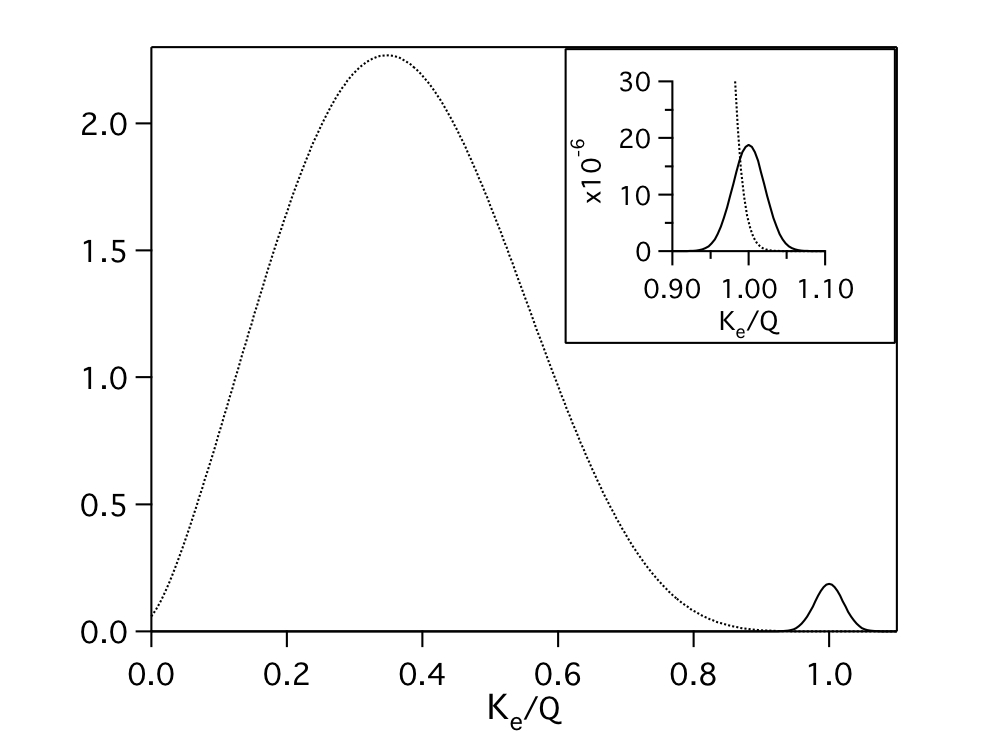
\includegraphics[scale=0.65]{pictures/Chap2/bbspectra.jpg}
\caption{Distribution of the sum of electron energies in case of 2$\nu\beta\beta$ (dashed line) and 0$\nu\beta\beta$ (solid line). The assumptions that $T_{\text{1/2}}^{\text{2}\nu}$ is 1~\% of $T_{\text{1/2}}^{\text{0}\nu}$ and the energy resolution is 2~\% have been done.}
\label{bbDecaySpectrum}
\end{center}
\end{figure}


\NI In the most general case, the half-life of 0$\nu\beta\beta$ is parametrised as : 


\begin{equation}
(\text{T}_{\text{1/2}}^{\text{0}\nu})^{\text{-1}} = \text{G}_{\text{0}\nu}\text{(Q}_{\beta\beta},\text{Z)} \times \text{M}^\text{2}_{\text{0}\nu} \times \eta^\text{2}
\end{equation}


\bigskip


\NI where G$_{\text{0}\nu}$ is a two-body phase space factor unlike G$_{\text{2}\nu}$ which is a four-body phase space factor. M$^\text{2}_{\text{0}\nu}$ is the 0$\nu\beta\beta$ NME and $\eta$ is a lepton violating number parameter which take into account all the physics behind 0$\nu\beta\beta$ mechanism. This parameter varies according the mechanism via which 0$\nu\beta\beta$ is mediated.  


\bigskip


\NI


\subsection{Effective mass of Majorana}


\NI The most commonly decay mode and which deviates the least from the SM is the neutrino mass mechanism. In this mechanism, 0$\nu\beta\beta$ is mediated by the light neutrino exchange. A Feynman diagram using only SM vertices can be drawn (Figure~\ref{0nubbFeynmanMassMechanism}), a right helicity Majorana neutrino is emitted from a W boson and absorbed by another as a left helicity Majorana neutrino.


\begin{figure}[h!]
\begin{center}
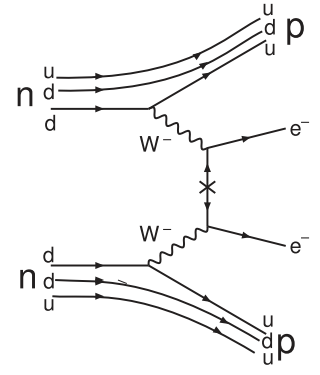
\includegraphics[scale=0.50]{pictures/Chap2/0nubbFeynmanMassMechanism.png}
\caption{aaa}
\label{0nubbFeynmanMassMechanism}
\end{center}
\end{figure}


\NI The change of helicity can happen only if the neutrino has a non-zero mass, the absorption by the  . In the Feynman diagram 


\ifx
La double désintégration β sans émission de neutrino qui viole de deux unités la
conservation du nombre leptonique est interdite par le Modèle Standard (voir le dia-
gramme figure 1.3). En effet, si l’on essaye d’en représenter le diagramme de Feynman
on se confronte à deux problèmes :
– différence particule-antiparticule : un ν  ̄ e émis depuis le vertex leptonique haut ne
peut pas être absorbé par celui du bas, celui-ci n’absorbant que des ν e ;
– différence d’hélicité : le lepton neutre émis d’en haut est d’hélicité positive et le
vertex du bas ne peut qu’absorber des leptons neutres d’hélicité négative


Cela nous impose d’avoir un neutrino qui satisfait à ν e = ν  ̄ e et m ν e = 0 (pour le
changement d’hélicité) afin que la double désintégration 2β0ν puisse avoir lieu. L’ampli-
tude du processus est alors proportionnelle à la masse de Majorana m ν e si on ne prend
pas en compte le mélange entre les neutrinos. Si on considère le mélange de neutrinos,
on obtient la masse de Majorana effective :
\fi
\bigskip

\begin{figure}[h!]
\begin{center}
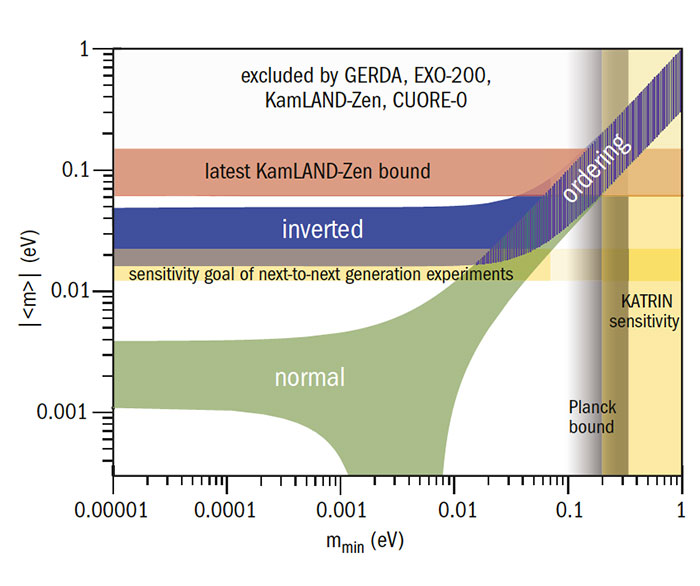
\includegraphics[scale=0.40]{pictures/Chap2/MeffVsMmin.jpg}
\caption{aaa}
\label{MeffVsMmin}
\end{center}
\end{figure}




\NI mettre ici le plot meff.



\NI explications , c'est interdit dans le MS, plot meff, ne pas oublier de spécifier que c'est relier avec les paramètres d'oscillations du neutrino.


\begin{figure}[h!]
\begin{center}
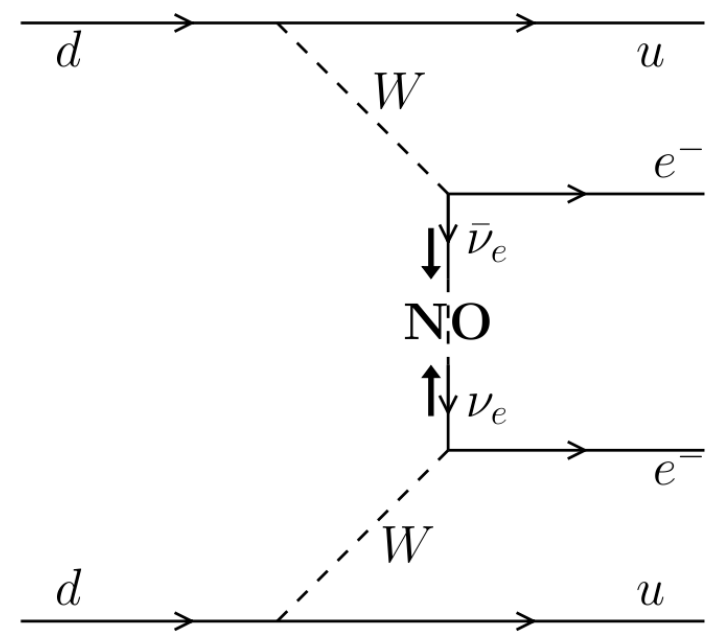
\includegraphics[scale=0.20]{pictures/Chap2/0nubb_Feynman.png}
\caption{Feynman diagram for 0$\nu\beta\beta$ decay. This process is forbidden in Standard Model because of the lepton number violation and have never been observed.}
\label{0nubbFeynman}
\end{center}
\end{figure}





\begin{figure}[h!]
\begin{center}
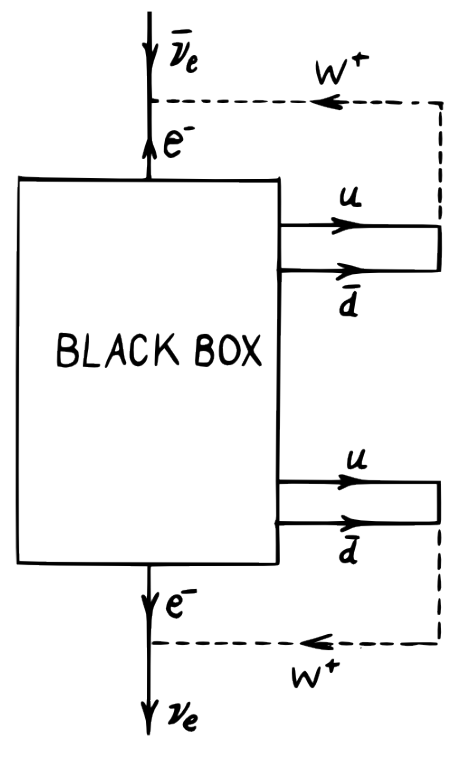
\includegraphics[scale=0.30]{pictures/Chap2/blackBox.png}
\caption{Black box showing that whatever the process behond the 0$\nu\beta\beta$ decay, its observation involves Majorana neutrinos.}
\label{blackBox}
\end{center}
\end{figure}



\begin{figure}[h!]
\begin{center}
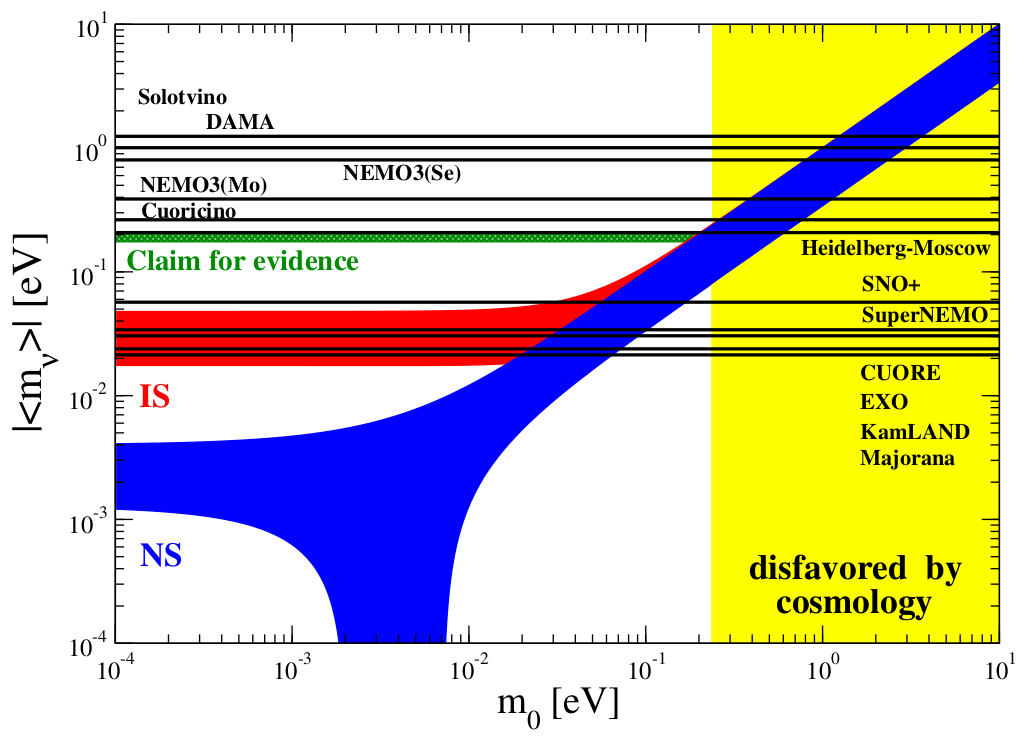
\includegraphics[scale=0.30]{pictures/Chap2/m_eff_neutrino.png}
\caption{Effective neutrino mass (|<m$_{\nu}$>| = m$_{\text{eff}}$) as a function of the lowest mass eigenstate (m$_\text{0}$). The blue and red regions represent the allowed values in Normal and Inverted Spectrum neutrino mass. The current experimental limits are also shown.}
\label{mEff}
\end{center}
\end{figure}



\NI Table~\ref{} summaries nuclides with the latest experimentally measured half-lives, (end of December 2016). 
 
 
 
 
 

\begin{equation}
\text{m} = \text{Z}.\text{m}_\text{p} + \text{(A - Z)}.\text{m}_{n} - \text{a}_\text{v} \text{A} + \text{a}_\text{s} \text{A}^{\text{2/3}} +  \text{a}_\text{c} \frac{\text{Z}^\text{2}}{\text{A}^{\text{1/3}}} +  \text{a}_\text{A} \frac{\text{(A-2Z)}^\text{2}}{\text{A}} + \delta \text{(A,Z)} 
\end{equation}

\NI where :


\begin{equation}
\delta \text{(A,Z)} = 
\left\{
\begin{array}{l}
  \frac{\text{a}_\text{p}}{\text{A}^{\text{1/2}}}~\text{Z,N~even~(A even)} \\[0.5cm]
  \text{0}~\text{A~odd}\\[0.5cm]
  -\frac{\text{a}_\text{p}}{\text{A}^{\text{1/2}}}~\text{Z,N~odd~(A even)} 
\end{array}
\right.
\end{equation} 




\begin{equation}
\text{m}_{\beta\beta} = |\sum_\text{i}U_{\text{ei}}^\text{2}~\text{m}_{\nu_\text{i}} |
\end{equation}






\subsection{Phenomenology}
\NI mettre la formule avec l'espace de phase, les éléments de matrices nucléaires et le éta. Dans le cas le plus simple, échange d'un neutrino léger de Majorana.



\subsection{Nuclear matrix elements}\label{sec:NME}

\subsection{Different isotopes}
\subsubsection{$^{\text{48}}$Ca}


\NI $^\text{48}$Ca is a rare isotope of calcium containing 20 protons and 28 neutrons. It is the lightest nucleus capable of 2$\nu\beta\beta$~decay. It can be considered as the golden isotope for $\beta\beta$ searches since it possesses the higher Q$_{\beta\beta}$ value (Q$_{\beta\beta}$ = 4.3~MeV) which is above almost all backgrounds. Unfortunately, its very low natural abundance (0.187~\%) limit its study at large exposure. Its 2$\nu\beta\beta$~decay rate have been measured by the NEMO-3 detector : T$_{\text{1/2}}^{\text{2}\nu}$ = 6.4 $^{\text{+0.7}}_{\text{-0.6}}$ (stat.) $^{\text{+1.2}}_{\text{-0.9}}$ (syst.) $\times$ 10$^{\text{19}}$ years. 

 
\subsubsection{$^{\text{76}}$Ge}


\NI $^\text{76}$Ge is an isotope of germanium containing 32 protons and 44 neutrons. Its natural abundance is approximately of 7~\%. Its low Q$_{\beta\beta}$ value (Q$_{\beta\beta}$ = 2.029~MeV) can be troublesome for the $\beta\beta$ searches. Its 2$\nu\beta\beta$~decay rate have been measured by the GERDA detector~:~T$_{\text{1/2}}^{\text{2}\nu}$ = 1.926 $\pm$ 0.094 $\times$ 10$^{\text{21}}$ years.   


\subsubsection{$^{\text{78}}$Kr}


\NI $^\text{78}$Kr is an isotope of krypton containing 36 protons and 42 neutrons. Its natural abundance is 0.36~\% . Its 2$\nu\beta\beta$~decay rate have been measured by the Baksan experiment~:~T$_{\text{1/2}}^{\text{2}\nu}$ = 9.2 $^{\text{+5.5}}_{\text{-2.6}}$ $\pm$ 1.3 $\times$ 10$^{\text{21}}$~years.   


\subsubsection{$^{\text{82}}$Se}


\NI $^\text{82}$Se is an isotope of selenium containing 34 protons and 48 neutrons. Its natural abundance is 8.82~\% and its Q$_{\beta\beta}$ value is 2.995~MeV. Its 2$\nu\beta\beta$~decay rate have been measured by the NEMO-3 detector~:~T$_{\text{1/2}}^{\text{2}\nu}$ = 10.07 $\pm$ 0.14 $\pm$ 0.54 $\times$ 10$^{\text{19}}$~years. 


\subsubsection{$^{\text{96}}$Zr}


\NI $^\text{96}$Zr is an isotope of zirconium containing 40 protons and 56 neutrons. Its natural abundance is 2.80~\% and its Q$_{\beta\beta}$ value is 3.348~MeV. Its 2$\nu\beta\beta$~decay rate have been measured by the NEMO-3 detector~:~T$_{\text{1/2}}^{\text{2}\nu}$ = 2.35 $\pm$ 0.14 $\pm$ 0.16 $\times$ 10$^{\text{19}}$~years.


\subsubsection{$^{\text{100}}$Mo}


\NI $^\text{100}$Mo is an isotope of molybdenium containing 40 protons and 56 neutrons. Its natural abundance is 9.74~\% and its Q$_{\beta\beta}$ value is 3.04~MeV. Its 2$\nu\beta\beta$~decay rate have been measured by the NEMO-3 detector~:~T$_{\text{1/2}}^{\text{2}\nu}$ = 7.1 $\pm$ 0.5 $\times$ 10$^{\text{18}}$~years and Ge coincidence~:~6.9 $^{\text{+1.0}}_{\text{-0.8}}$ $\pm$ 0.7 $\times$ 10$^{\text{18}}$~years.


\subsubsection{$^{\text{116}}$Cd}


\NI $^\text{116}$Cd is an isotope of cadmium containing 48 protons and 68 neutrons. Its natural abundance is 7.51~\% and its Q$_{\beta\beta}$ value is 2.809~MeV. Its 2$\nu\beta\beta$~decay rate have been measured by the NEMO-3 detector~:~T$_{\text{1/2}}^{\text{2}\nu}$ = 2.74 $\pm$ 0.04 $\pm$ 0.18 $\times$ 10$^{\text{19}}$~years and by Elegant : 2.6 $^{\text{+0.9}}_{\text{-0.5}}$ $\times$ 10$^{\text{18}}$~years.


\subsubsection{$^{\text{128}}$Te}


\NI $^\text{128}$Te is an isotope of tellerium containing 52 protons and 76 neutrons. Its natural abundance is 31.74~\% and its Q$_{\beta\beta}$ value is 0.867. Its 2$\nu\beta\beta$~decay rate have been measured by geochemical method~:~T$_{\text{1/2}}^{\text{2}\nu}$ = 2.2 $\times$ 10$^{\text{24}}$~years which is the longest half-life of all isotopes proven to be radioactive.


\subsubsection{$^{\text{130}}$Te}


\NI $^\text{130}$Te is an isotope of tellerium containing 52 protons and 78 neutrons. Its natural abundance is 34.08~\% and its Q$_{\beta\beta}$ value is 2.528~MeV. Its most precise measurement of 2$\nu\beta\beta$~decay rate have been measured by CUORE-0~:~T$_{\text{1/2}}^{\text{2}\nu}$ = 8.2 $\pm$ 0.2 $\pm$ 0.6 $\times$ 10$^{\text{20}}$~years.


\subsubsection{$^{\text{136}}$Xe}


\NI $^\text{136}$Xe is an isotope of xenon containing 54 protons and 82 neutrons. Its natural abundance is 8.8573~\% and its Q$_{\beta\beta}$ value is 2.458~MeV. Its 2$\nu\beta\beta$~decay rate have been measured by EXO-200~:~T$_{\text{1/2}}^{\text{2}\nu}$ = 2.165 $\pm$ 0.016 $\pm$ 0.059 $\times$ 10$^{\text{20}}$~years.


\subsubsection{$^{\text{150}}$Nd}


\NI $^\text{150}$Nd is an isotope of neodynium containing 60 protons and 90 neutrons. Its natural abundance is 5.6~\% and its Q$_{\beta\beta}$ value is 3.367~MeV. Its 2$\nu\beta\beta$~decay rate have been measured by NEMO-3~:~T$_{\text{1/2}}^{\text{2}\nu}$ = 9.34 $\pm$ 0.22 $^{\text{+0.62}}_{\text{-0.60}}$ $\times$ 10$^{\text{18}}$~years.


\subsubsection{$^{\text{238}}$U}
\NI 


\NI It exists 41 naturally isotopes capable of 2$\nu\beta\beta$~decay (35 of $\beta^{-}$ and 6 of $\beta^{+}$ decays). Today 12 isotopes have been experimentally observed undergoing 2$\nu\beta\beta$~decay. \textcolor{red}{dire que c'est un émetteru alpha avec une longue demi vie et que la double beta est possible}


\begin{figure}[h!]
\begin{center}
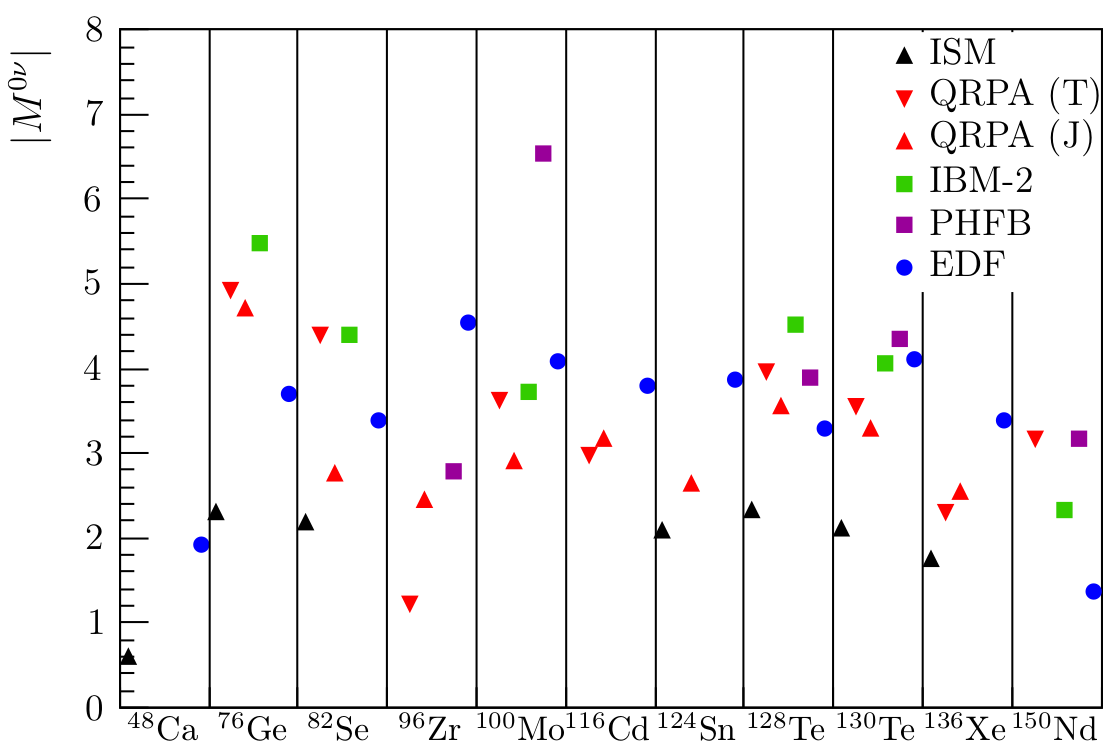
\includegraphics[scale=0.30]{pictures/Chap2/NMEdetailes.png}
\caption{Summary of 0$\nu\beta\beta$ Nuclear Matrix Element (NME) computations, calculated for 11 isotopes, using different approaches. These results are extracted from \cite{TheoryOfNeutrinolessDBD}, conversion for g$_{\text{A}}$ = 1.25 and r$_{\text{0}}$  = 1.2~fm have been made if necessary.}
\label{NME}
\end{center}
\end{figure}



\subsection{Other processes behond $\beta\beta0\nu$}

\NI

\ifx
There are many different hypothesised mechanisms via which 0νββ may be mediated,
the most common of which are the neutrino mass mechanism, right-handed current
and Majoron emission modes (Sections 3.3.1–3.3.3). There also exist a plethora of
more exotic decay modes such as via R-parity violating super-symmetry, squark
mixing or extra dimensions which are not presented herein.
For some mechanisms, such as the mass mechanism, it is readily apparent that 0νββ
confirms that neutrinos are Majorana paricles. In constrast, for some of the more
exotic decays where neutrinos are not involved at all, such as in R-parity violating
SUSY [33], things are not so obvious. The situation was clarified by Schechter and
Valle in 1980, who showed that any 0νββ process implies that neutrinos are Majorana
particles [34]. This can be seen by replacing the 0νββ mechanism with a “Black Box”
(Figure 3.3) and confirming that there exists a propagator that converts between
neutrinos and antineutrinos as is required for a Majorana mass (Section 2.3.2).
\fi

\begin{figure}[h!]
\begin{center}
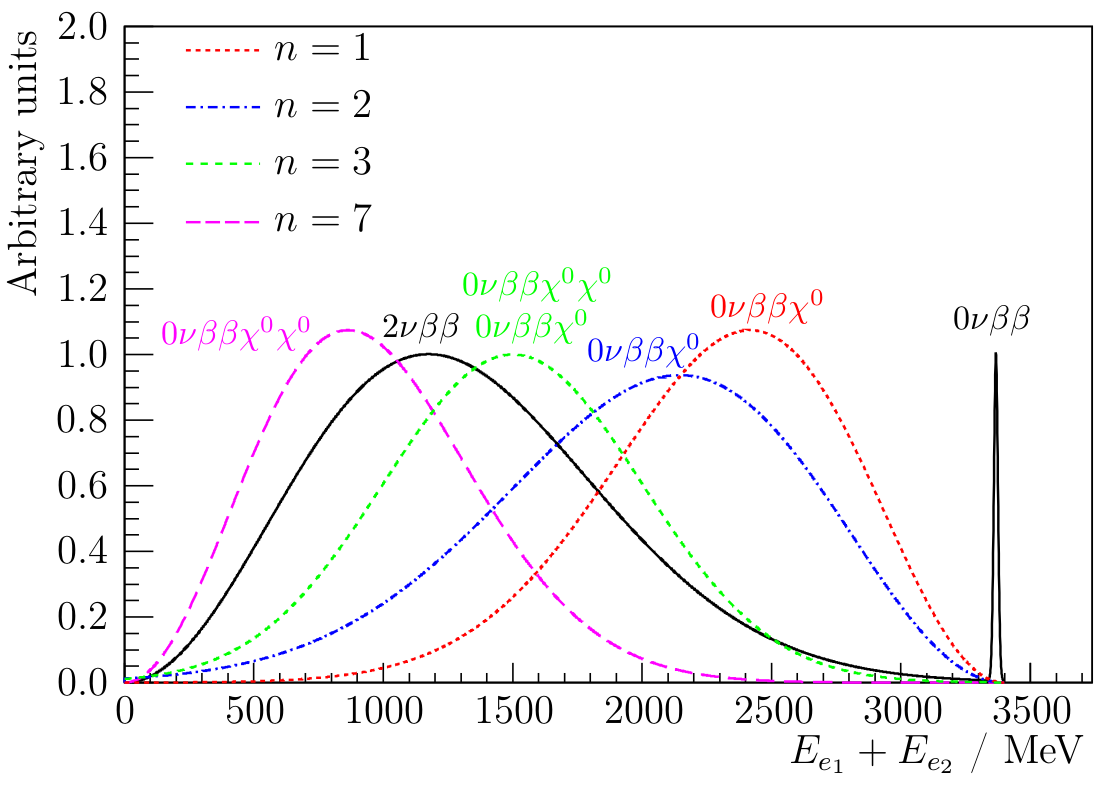
\includegraphics[scale=0.30]{pictures/Chap2/SpectrumFifferentMechanism.png}
\caption{Distribution of the sum of electron energies for 2$\nu\beta\beta$ and 0$\nu\beta\beta$ according different Majoron decay modes with spectal indices 1,2,3 and 7.}
\label{DifferentbbDecaySpectrum}
\end{center}
\end{figure}



\section{Experimental point of view}\label{sec:ExperimentalSearches}
\NI mettre formule sens, il faut des détecteurs bas bruit de fond, ... radiopureté ... parler de l'efficacité,
\NI deux approches sont aujourd'hui considérés : tracko calo et juste calo. Point fort et point faible de chaque approche


\section{Status of double beta experiments}\label{sec:Status0nubb}
\NI Faire un statut de la double beta aujourd'hui avec 
\NI Gerda, KamLandZen, Cuore.
\subsection{KamLAND-Zen}
\subsection{GERDA}
\subsection{Cuore}
\end{document}
